% !TeX root = ../main.tex

\chapter{补充材料}


\section{实验图表}


实验中的部分图表如下,图表标题的格式为“(noise\_ratio,outliers\_ratio)-数据集名称 损失函数比/加速比”。
虚线表示未使用核心集框架的情况,实线表示使用了核心集框架的情况,相同颜色的线表示相同的核心集方法。
可以看到MNIST数据集在两种不同参数的情况下,表现差距较大。
\begin{figure}
    

\centering
    \begin{minipage}{0.49\linewidth}
        \centering
        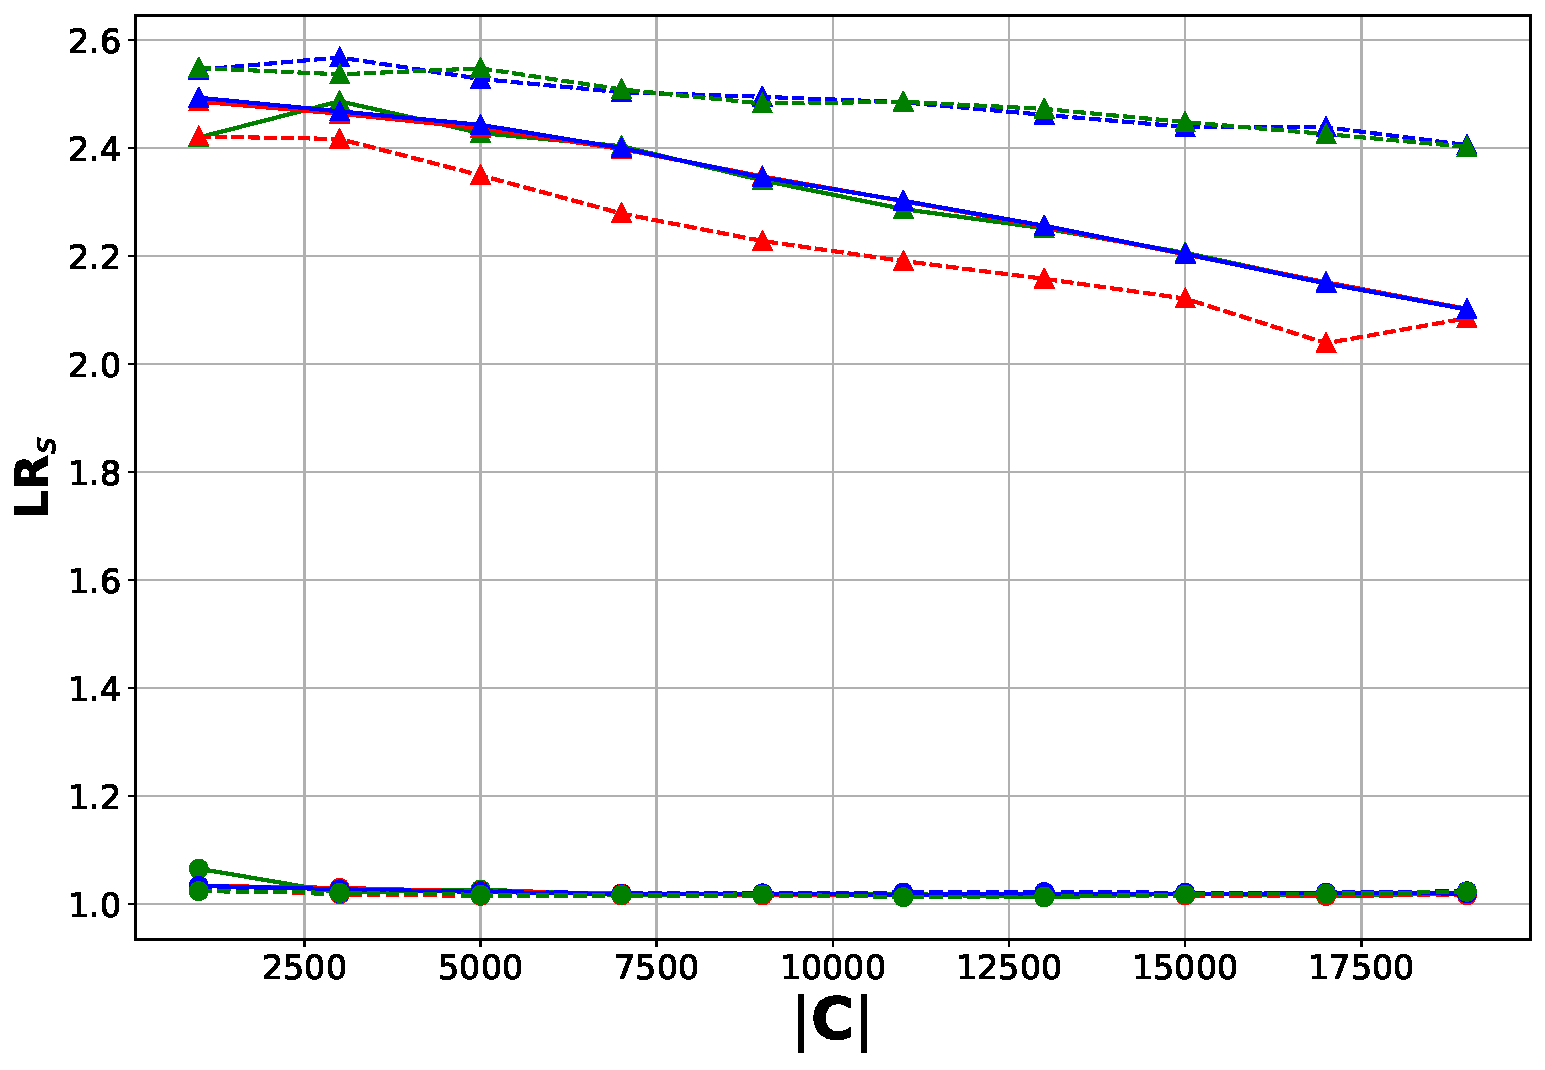
\includegraphics[width=\linewidth]{./fig/loss_ratio(0.05,0.2) - MNIST.pdf}
        \subcaption{(0.05,0.2)-MNIST $\mathbf{LR},\mathbf{LR}_z$}
    \end{minipage}
    \hfill
    \begin{minipage}{0.49\linewidth}
        \centering
        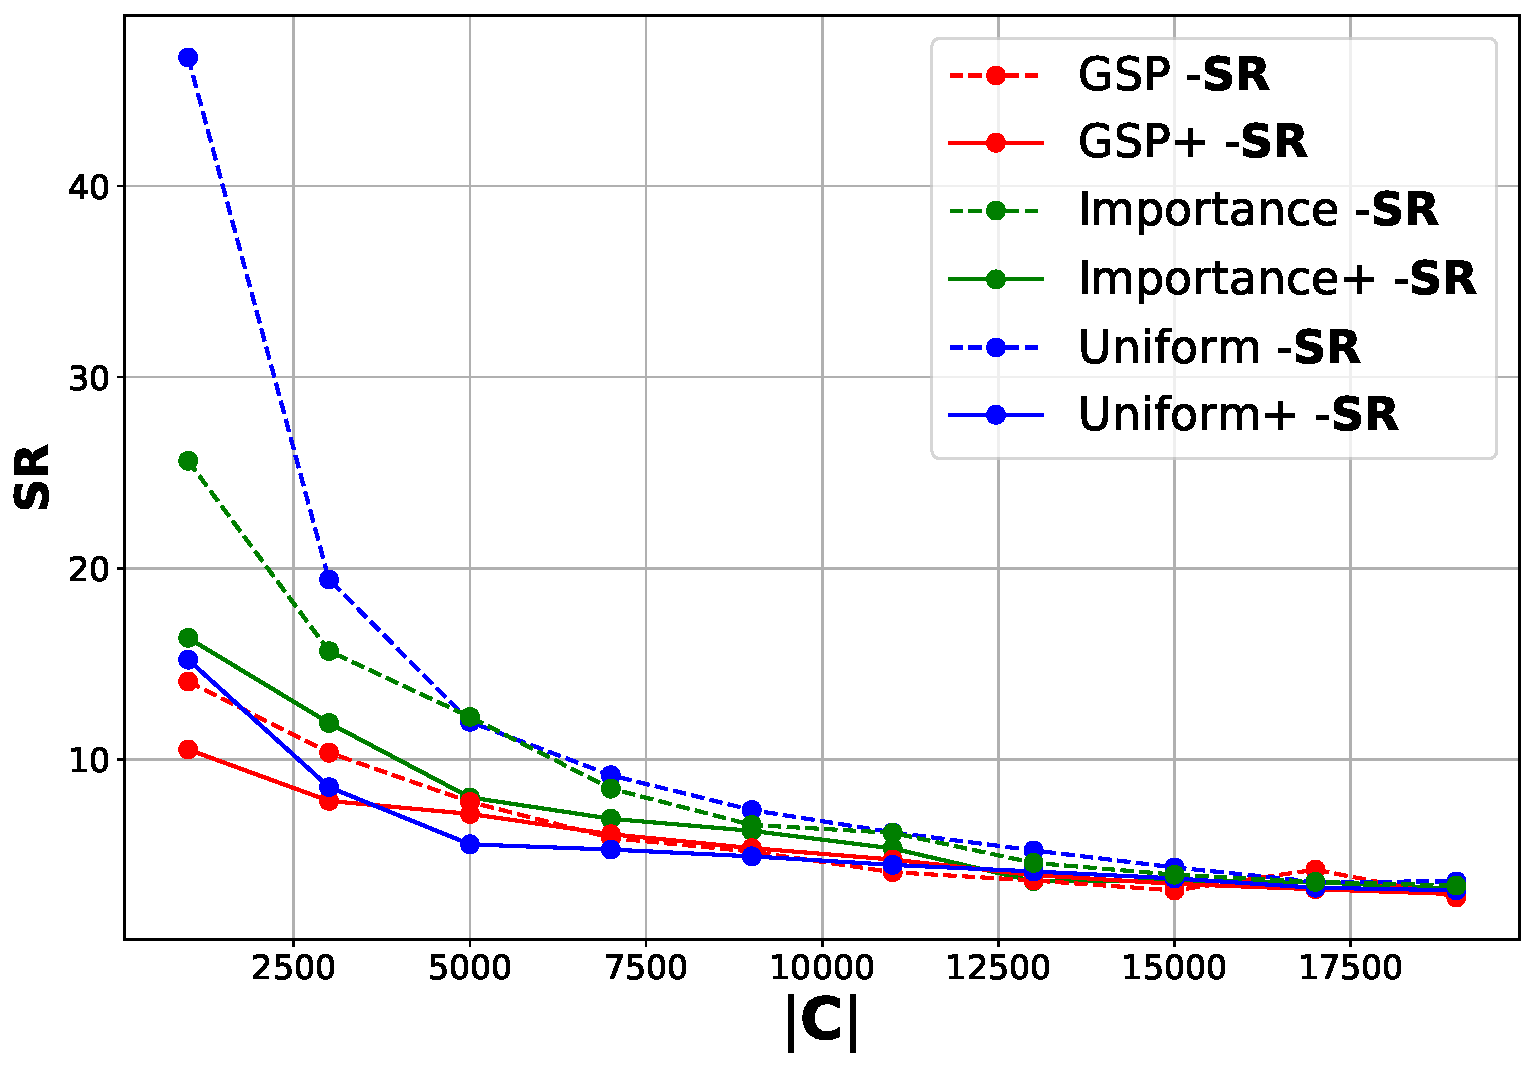
\includegraphics[width=\linewidth]{./fig/time_ratio(0.05,0.2) - MNIST.pdf}
        \subcaption{(0.05,0.2)-MNIST $\mathbf{SR}$}
    \end{minipage}
    \\
    \begin{minipage}{0.49\linewidth}
        \centering
        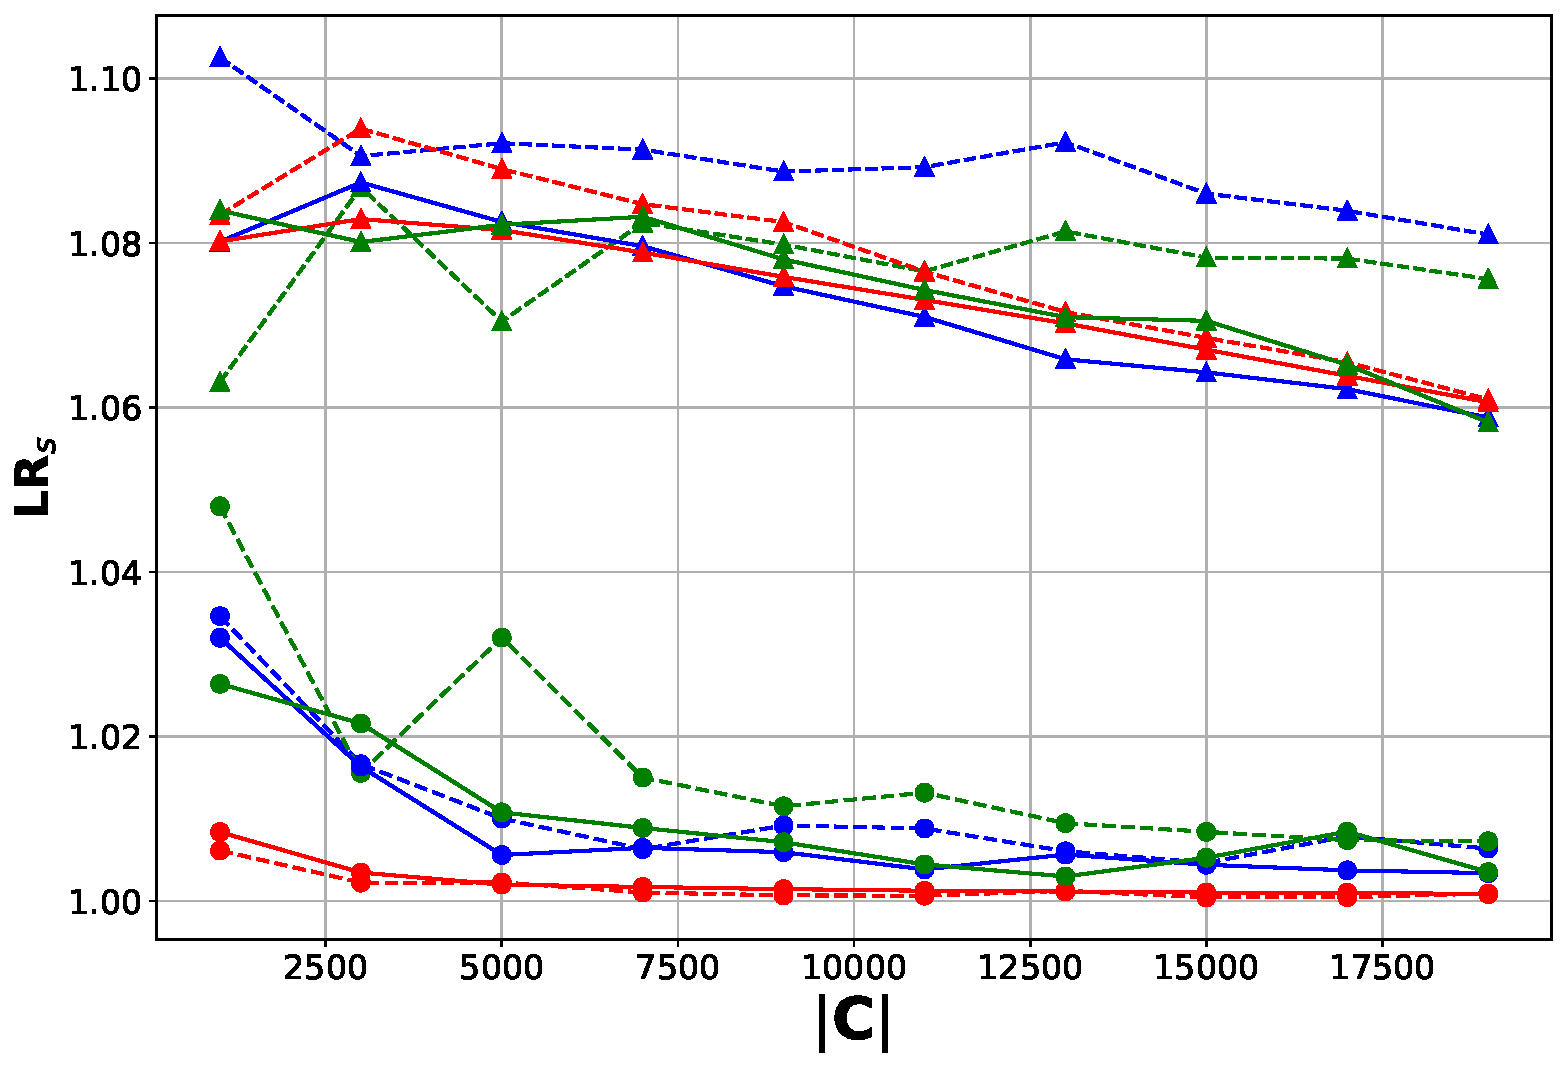
\includegraphics[width=\linewidth]{./fig/loss_ratio(0.2,0.05) - MNIST.pdf}
        \subcaption{(0.2,0.05)-MNIST $\mathbf{LR},\mathbf{LR}_z$}
    \end{minipage}
    \hfill
    \begin{minipage}{0.49\linewidth}
        \centering
        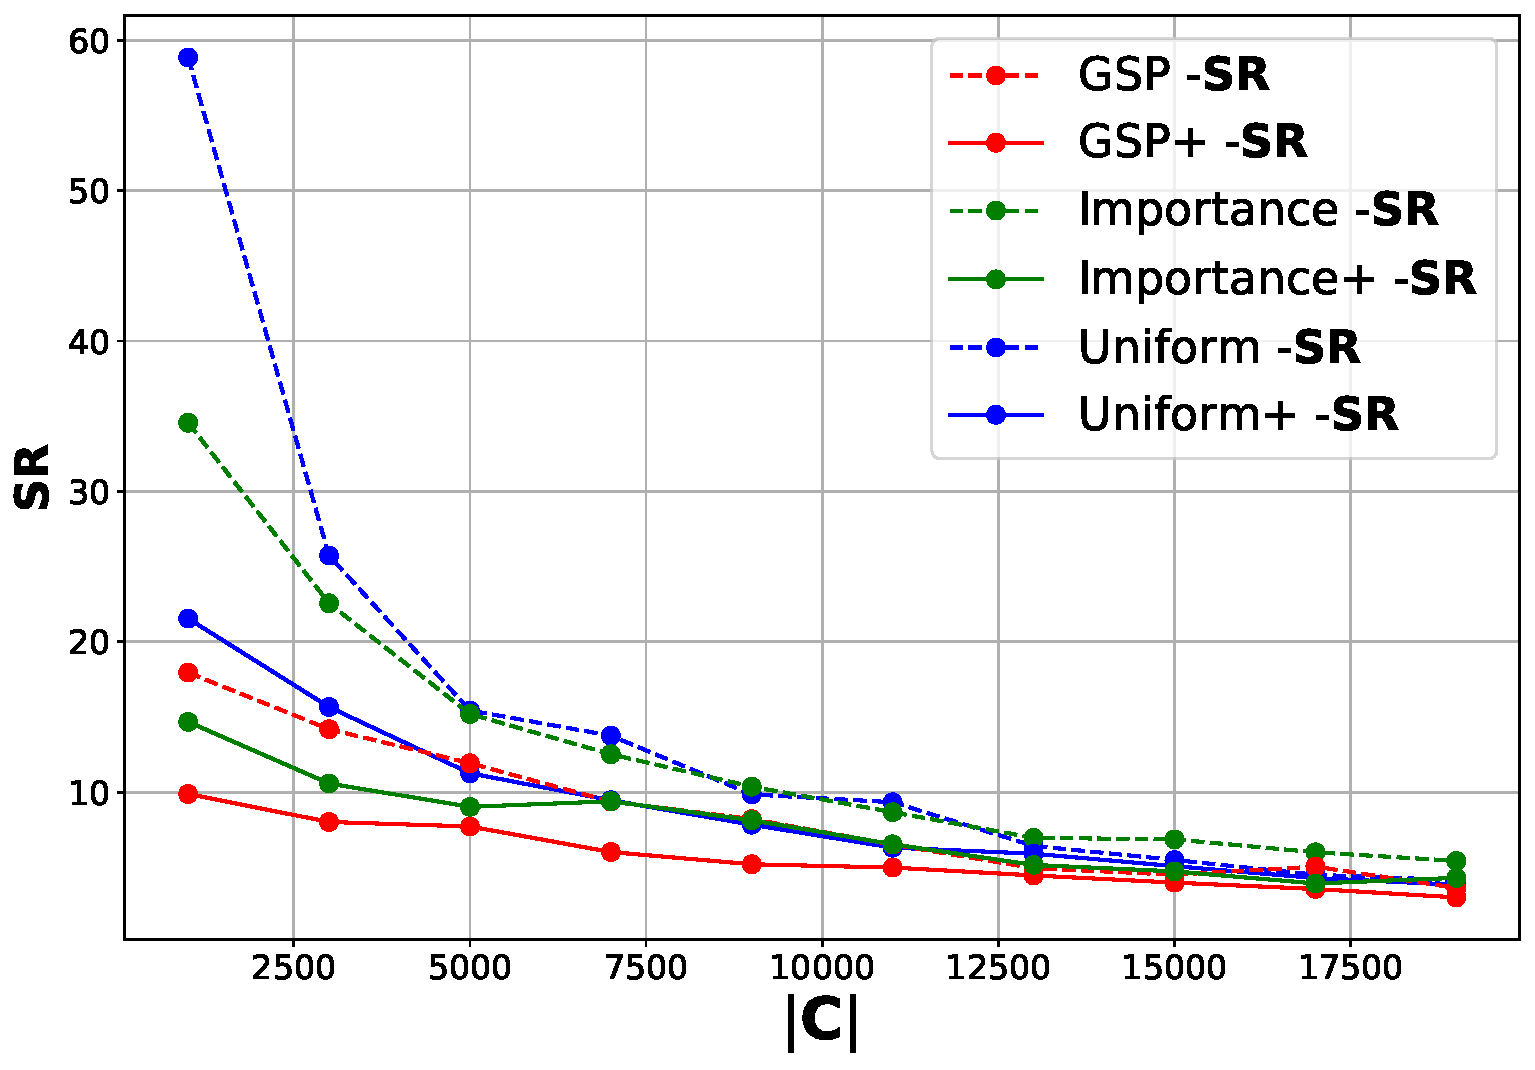
\includegraphics[width=\linewidth]{./fig/time_ratio(0.2,0.05) - MNIST.pdf}
        \subcaption{(0.2,0.05)-MNIST $\mathbf{SR}$}
    \end{minipage}
    \\
    \begin{minipage}{0.49\linewidth}
        \centering
        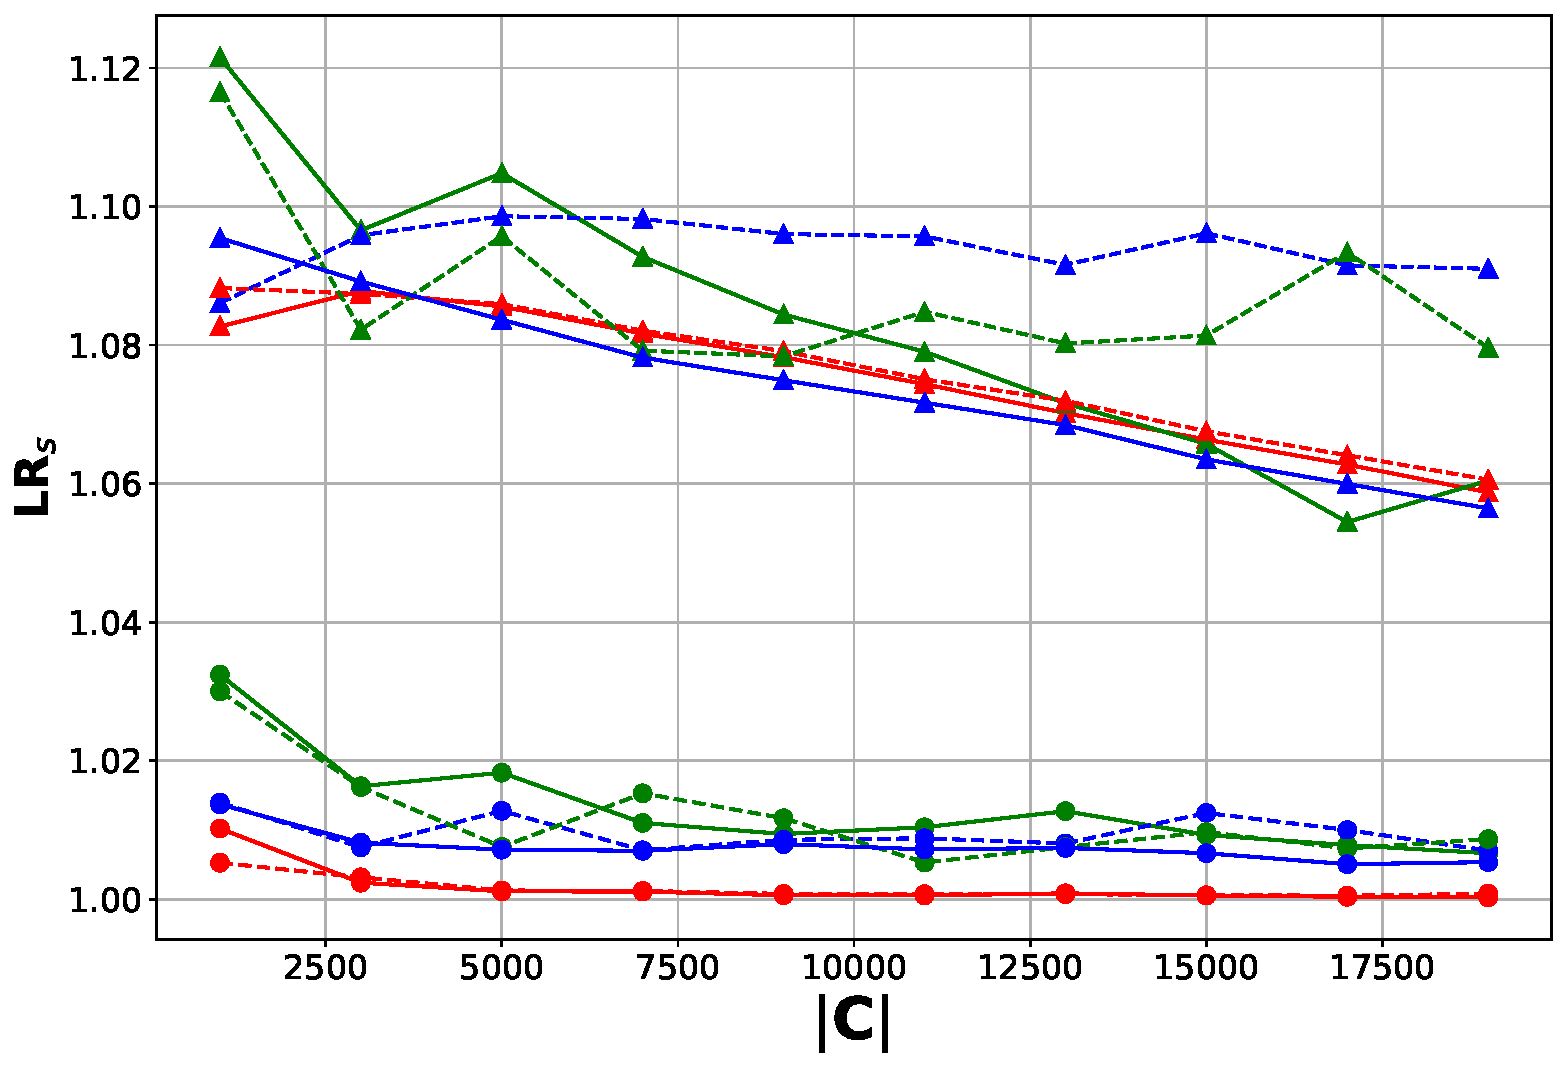
\includegraphics[width=\linewidth]{./fig/loss_ratio(0.2,0.05) - CIFAR-10.pdf}
        \subcaption{(0.2,0.05)-CIFAR-10 $\mathbf{LR},\mathbf{LR}_z$}
    \end{minipage}
    \hfill
    %\hspace{0.005\linewidth}
    \begin{minipage}{0.49\linewidth}
        \centering
        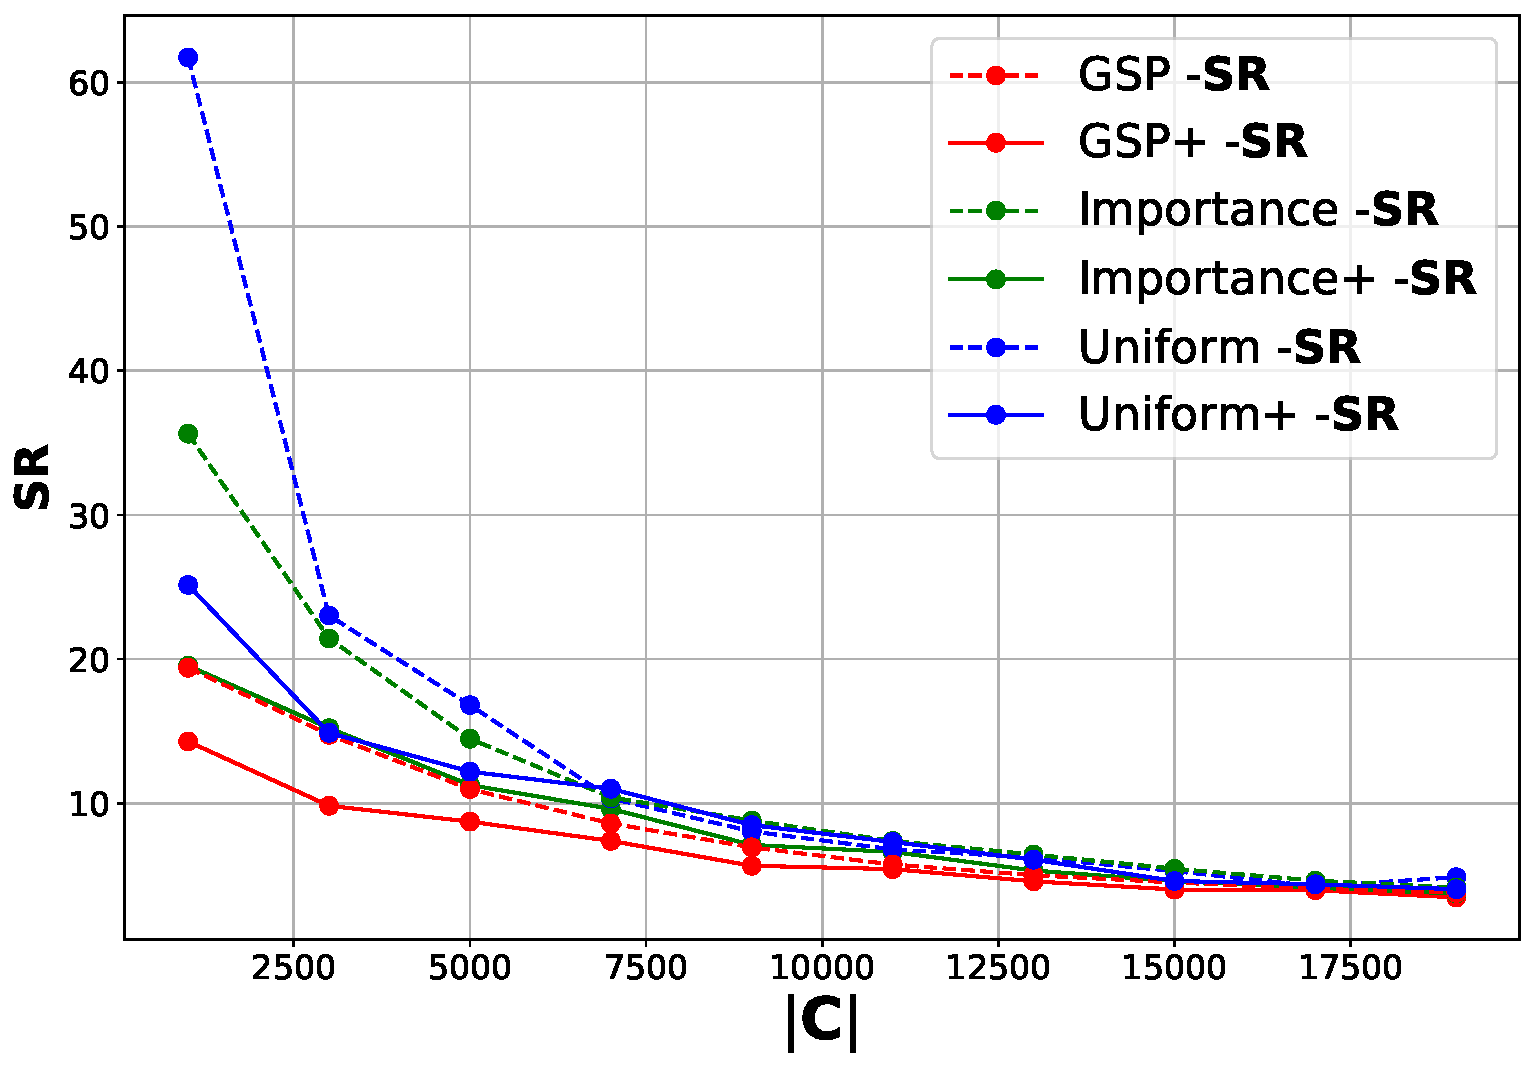
\includegraphics[width=\linewidth]{./fig/time_ratio(0.2,0.05) - CIFAR-10.pdf}
        \subcaption{(0.2,0.05)-CIFAR-10 $\mathbf{SR}$}
    \end{minipage}
    \caption{实验图一}
\end{figure}
    




\begin{figure}[!htbp]
    
    \begin{minipage}{0.49\linewidth}
        \centering
        \includegraphics[width=\linewidth]{./fig/loss_ratio(0.001,0.02) - Covertype.pdf}
        \subcaption{(0.001,0.02)-Covertype $\mathbf{LR}$}
    \end{minipage}
    \hfill
    %\hspace{0.005\linewidth}
    \begin{minipage}{0.45\linewidth}
        \centering
        \includegraphics[width=\linewidth]{./fig/time_ratio(0.001,0.02) - Covertype.pdf}
        \subcaption{(0.001,0.02)-Covertype $\mathbf{SR}$}
    \end{minipage}
    \\
    \begin{minipage}{0.45\linewidth}
        \centering
        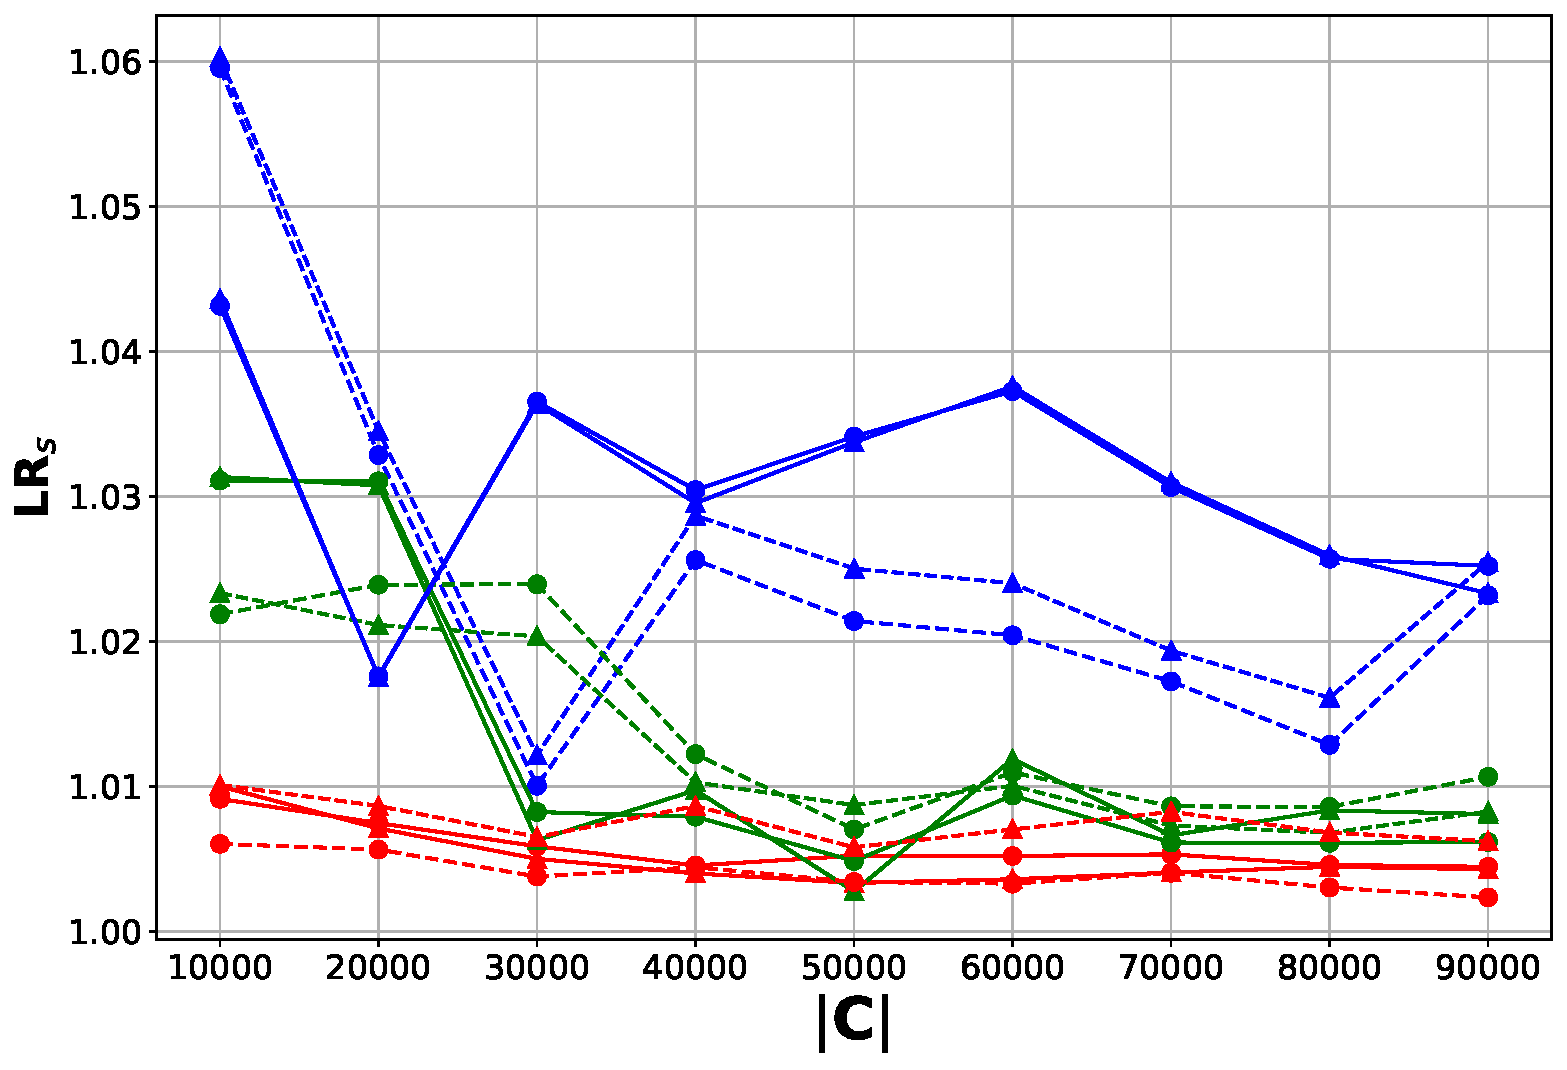
\includegraphics[width=\linewidth]{./fig/loss_ratio(0.01,0.0001) - USCensus.pdf}
        \subcaption{(0.01,0.0001)-USCensus $\mathbf{LR}$}
    \end{minipage}
    \hfill
    %\hspace{0.005\linewidth}
    \begin{minipage}{0.45\linewidth}
        \centering
        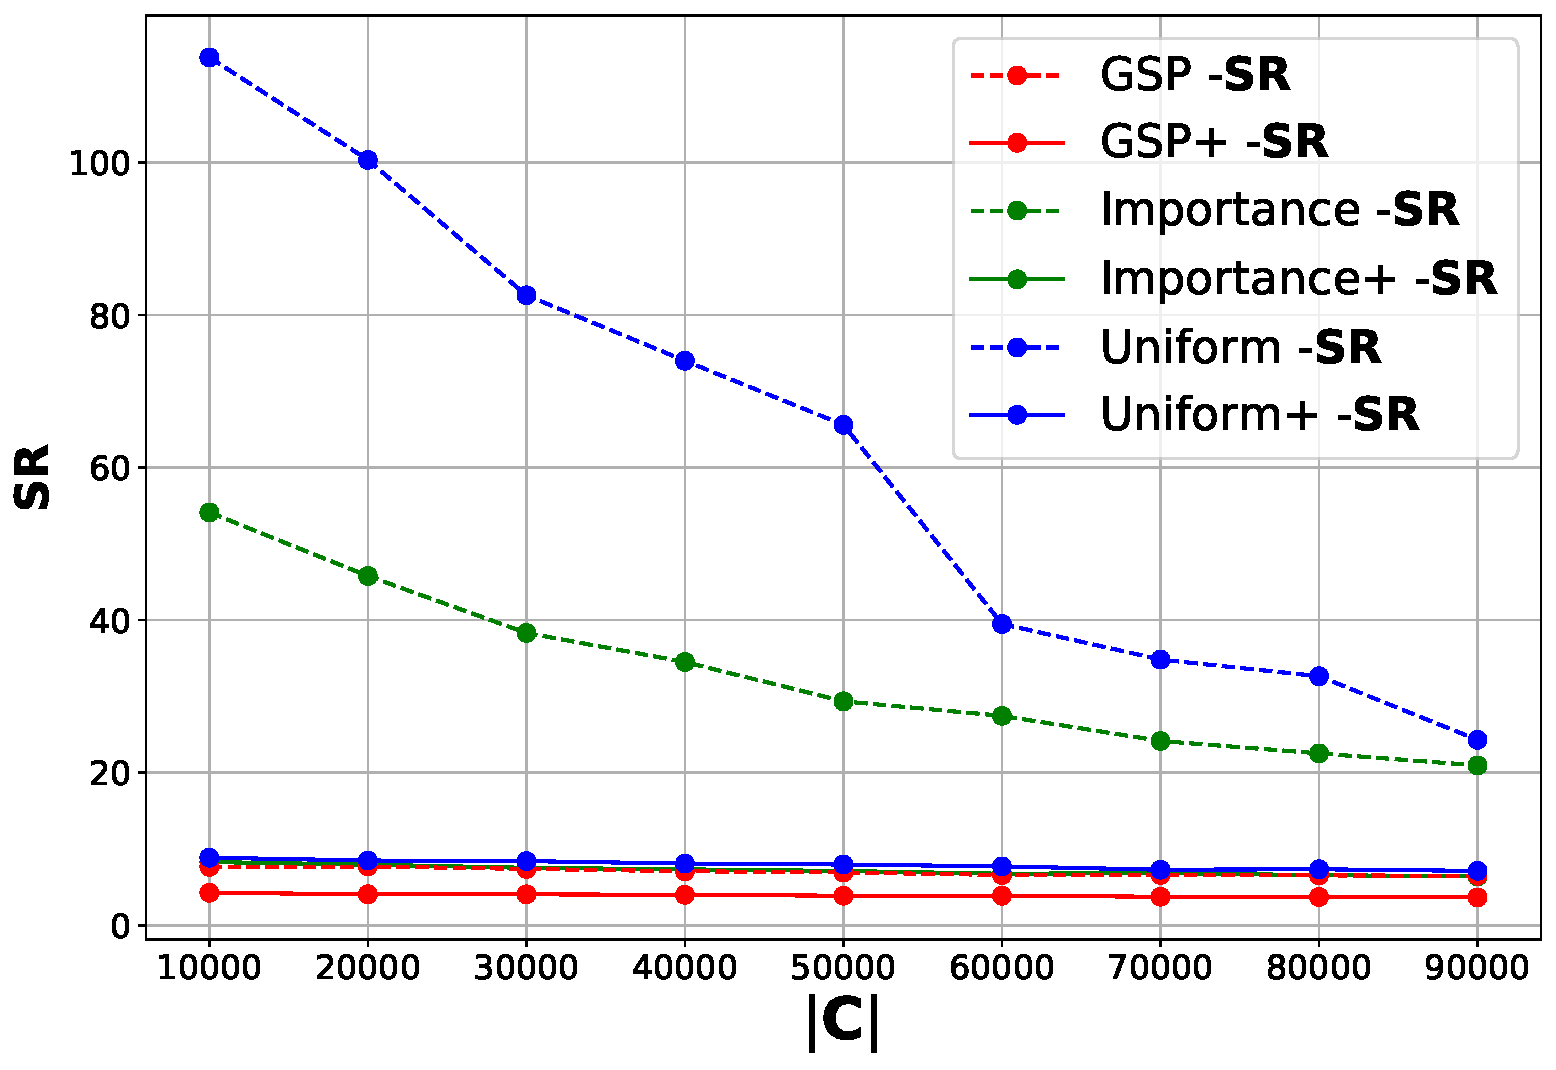
\includegraphics[width=\linewidth]{./fig/time_ratio(0.01,0.0001) - USCensus.pdf}
        \subcaption{(0.01,0.0001)-USCensus $\mathbf{SR}$}
    \end{minipage}
    
    \caption{实验图二}
\end{figure}


